% !TeX root = ../main.tex
% Add the above to each chapter to make compiling the PDF easier in some editors.

\chapter{Preliminaries}\label{chapter:introduction}
In this chapter, we introduce the mathematical notations and preliminaries used for the whole thesis. Firstly, the coverage control is formulated analytically to demonstrate the goal of the control method. The agents considered in this thesis are Wheeled Mobile Robots (WMRs), we also introduce the standard nonlinear dynamic of WMR afterwards. 

\section{Notations}
\begin{tabular}{ l l }
	${\mathbb{R}}$ & Set of real numbers  \\
	${\mathbb{R}_+}$ & Set of non-negative real numbers  \\
	${\mathbb{C}}$ & Set of complex numbers \\
	${i = \sqrt{-1}}$ & The imaginary unit \\
	${\Re (z)}$ & Real part of ${z \in \mathbb{C}}$ \\
	${\Im (z)}$ & Imaginary part of ${z \in \mathbb{C}}$ \\
	${\bar{z}}$ & The complex conjugate of ${z \in \mathbb{C}}$ \\
	${\langle z_1,z_2  \rangle = \Re(\bar{z_1}z_2)}$ & Scalar product of ${z_1, z_2 \in \mathbb{C}}$ \\
	%${}$ & \\
	%${}$ & \\
	%${}$ & \\
\end{tabular}
\section{Voronoi Coverage Control}
The problem of coverage control is to deploy a group of multiple agents to cover a specific area. This general concept is well defined in the pioneering works [2], [3]. In the above-mentioned publications, MAS use the coverage control method to obtain an optimal sensing capability, which means they can robustly capture any events within a specific region. There are many kinds of formation which depends on the the art of coverage. Firstly, this section will introduce the Voronoi tessellations and later on will depict the relation between of this topology and the sensing performance of agents.

\subsection{Voronoi Tessellations}
Define a region ${Q: \{q \in \mathbb{R}^2\}}$ and ${n}$ arbitrary points ${Z = \{z_1, z_2, ..., z_n\} \in \mathbb{R}^2 }$ inside this region. These points are called the generator of Voronoi tesselation and they divide the region ${Q}$ into n partitions ${V_k \txtspc{,} k \in \{1,...,n\}}$ that satisfy \\ 
\begin{equation}
\begin{split}
V_k & = \{q \in Q \txtspc{|} \norm{q-z_k} \leq \norm{q-z_j} \} \\
Q & = V_1 \cup V_2 \cup ... \cup V_n
\end{split}
\end{equation}

\noindent Figure \ref{fig:Voronoi_Tessellation} depicts the Voronoi partitions constructed inside a bounded region.

\begin{figure}[!htb]
	\centering
	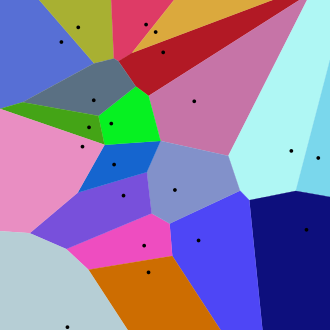
\includegraphics[width=0.4\textwidth]{voronoi_tesselation}
	\caption{Voronoi Tessellations}
	\label{fig:Voronoi_Tessellation}
\end{figure}
\[source: https://en.wikipedia.org/wiki/Voronoi\_diagram\]

\begin{figure}[!htb]
	\centering
	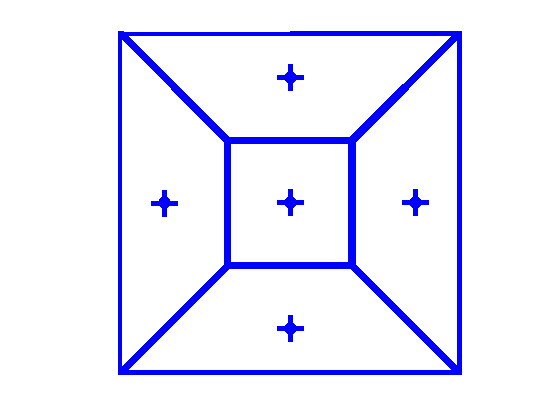
\includegraphics[width=0.4\linewidth]{CentroidalVoronoiTessellation3}
	\label{fig:CentroidalVoronoiTessellation}
	\caption{Centroidal Voronoi Tessellations}
\end{figure} 	
\[source:https://en.wikipedia.org/wiki/Centroidal\_Voronoi\_tessellation\]

\subsection{Centroidal Voronoi Tessellations}
A special type of Voronoi tessellation is a centroidal Voronoi tessellation (CVT). This configuration has the characteristic that the generator points are also the central mass of each partition. Figure 2.2 shows an example of a CVT.

\subsection{Optimization of Sensing Capability}
In coverage control, a group of ${n}$ agents with onboard sensors has to cover a region ${Q \in \mathbb{R}^2}$. Define a distribution density function ${\phi(q): Q \rightarrow \mathbb{R}_+}$, this function determines the chance that an event would happen at a specific region in Q. The location of agents is described as vector notation ${Z = (z_1, z_2, ..., z_n) \in \mathbb{R}^n}$. The performance of the attached sensors on each agent relates to the physical characteristic, such as ultrasonic or light sensors. The sensing capability is inverse proportional to the distance between sensor location and the events in the detectable area. This means the closer one sensor is located to the events that tend happen, the more efficient the performance will be. Therefore, we define a positive, increasing function ${f(\norm{q - z_k})}$ to represent how poor the performance of sensors in relation to the distance of measurement. The standard cost function proposed in [2],[3] for the sensing performance is considered as\\
\begin{equation}
H(Z) = \displaystyle \int_{Q} \underset{k \in {1,...,n}}{\normalfont{min}} f(\norm{q - {z_{k}}}) \phi(q) \mathrm{d}q \label{general_cost_function}
\end{equation}
From the introduction of Voronoi Tessellations in the previous subsection, we can see from the cost function that the performance of the whole system depends on the position of each agent to maximize the sensing capability within its own region. The cost function is reformulated as 
\begin{equation}
H(Z) = \displaystyle\sum_{k=1}^{n}  \int_{V_{k}}  f(\norm{q - {z_{k}}}) \phi(q) \mathrm{d}q \label{voronoi_cost_function}
\end{equation}

%\[ \norm{a \vec{u}} = \abs{a} \, \norm{\vec{v}} \]
\noindent In order to maximize the sensing capability of MAS, we minimize the cost function (\ref{voronoi_cost_function}). Let ${f(\norm{q - {z_{k}}}) = \frac{1}{2}\norm{q-z_k}^2}$ as a strictly increasing, differentiable function. We determine the optimal point of (\ref{voronoi_cost_function}) through gradient of H(Z) as following: \\
\textbf{Lemma 1. (Lemma 2.1, Schwager (2009))} \\ 
%From z = [z_{1} z_{2} ... z_{k}], where k is the amount of agent
\begin{equation} \notag
\begin{split}
\frac{\partial H(Z)}{\partial {z_k}} &  = \displaystyle\sum_{k=1}^{n} \int_{V_{k}} \frac{\partial }{\partial {z_{k}}}  \frac{1}{2}\norm{q - {z_{k}}}^2 \phi(q) \mathrm{d}q \\
& = \displaystyle\sum_{k=1}^{n} (z_{k} \int_{V_{k}} \phi(q) \mathrm{d}q - \int_{V_{k}} q \phi(q) \mathrm{d}q) \\   
\end{split}
\end{equation}
\noindent By defining  
\[M_{V_{k}} = \int_{V_{k}} q \phi(q) \mathrm{d}q\] 
\[C_{V_{k}} = \frac{1}{M_{V_{k}}} \int_{V_{k}} q \phi(q) \mathrm{d}q\]

\noindent we have 
\begin{equation} \label{optimal_comndition}
\frac{\partial H(Z)}{\partial {z_k}} = \displaystyle\sum_{k=1}^{n} M_{V_{k}}(z_{k} - C_{V_{k}})
\end{equation}

\noindent The gradient of (\ref{voronoi_cost_function}) is thought to be complex because the boundaries of each region are also related to the adjacent regions. What Schwager did in his Lemma 2.1 pointed out that the complex terms of the boundary points eliminate each other and result in a simple function that the optimum location of each agent $z_k$ only depends on the geometry of the region ${V_k}$ . Interested readers may refer to [3] to understand more about the way Schwager performed the derivative under the integral sign. Moreover, the dynamics of Voronoi partitions are studied in previous works [12],[13],[14],[19].
\noindent From (\ref{optimal_comndition}), the cost function achieves its local optimum if and only if all generators converge on the set of centroidal Voronoi configuration. This motivates us to design the control policy for agents to approach this configuration.

\section{Non-holonomic Wheeled Mobile Robot Model}
\noindent The agents considered in this thesis are non-holonomic wheeled mobile robots (WMRs) that have non-linear dynamic. Each agent has a non-identical fixed translation velocity ${v_k \in \mathbb{R}_{+}}$ and a rotation velocity ${u_{k}}$. When a WMR moves, we define a unique virtual mass which is related to the control input and its actual states. We formulate the dynamic of a WMR and its virtual mass as follows\\ 
\noindent $\bullet$ Dynamics of WMR % in Cartesian coordinate system
\begin{equation} \label{WMR_dynamic}
\begin{split}
\dot{x}_{k} & = v_{k} cos(\theta_{k})  \\
\dot{y}_{k} & = v_{k} cos(\theta_{k})  \\
\dot{\theta}_{k} & = u_{k} \\
\end{split}
\end{equation}

\noindent Let $r_k \in \mathbb{C}:\txtspc{ }r_k = x_k + iy_k $, the above dynamic can be formulated in complex notation as 
\begin{equation} \notag
\begin{split}
\dot{r}_{k} & = v_{k} e^{i \theta_{k}} \\
\dot{\theta}_{k} & = u_{k} \\
\end{split}
\end{equation}
\noindent The complex notation $z_k$ determines the virtual mass of an agent as
\[z_k = r_k + \frac{v_k}{w_0}ie^{i\theta_{k}}\]

\noindent $\bullet$  Dynamic of WMR's virtual mass %in Cartesian coordinate system
\begin{equation} \label{VM_dynamic}
\begin{split}
\dot{z}_{k} = v_k e^{i\theta_{k}} - \frac{v_k}{w_0}e^{i\theta_{k}}u_k \\
\end{split}
\end{equation}



\section{Problem Statement}
\noindent Given ${n}$ wheeled mobile robots with vector ${Z = (z_1, z_2,..., z_n) \in \mathbb{C}^n}$ denotes the location of each agent's virtual mass. Each agent has  a non-identical constant translation velocity $v_k$. For a predefined convex region ${Q = \{q \in \mathbb{R}^2 \txtspc{|} Aq \leq b\}}$, ${A \in \mathbb{R}^{m \times 2} \txtspc{,} b \in \mathbb{R}^m}$, where ${m}$ is the amount of boundary lines that cover the region ${Q}$, find the control law ${U = (u_1, u_2,..., u_n) \in \mathbb{R}^n }$ for all agents to orbit the set of Centroidal voronoi Configuration in $Q$ and always satisfy the hard constraints:\\
\[A[\Re{(z_k(t))} \txtspc{ } \Im{(z_k(t))}]^T \leq b \txtspc{,} \forall k \in \{1,...,n\} \txtspc{,} \forall t\]
\[u_k(t) \in [-U_{k_{low}}\txtspc{ } U_{k_{up}}]\txtspc{,} \forall k \in \{1,...,n\} \txtspc{,} w_{k_0} \in [-U_{k_{low}} \txtspc{ } U_{k_{up}}] , U_{k_{low}},U_{k_{up}} \in \mathbb{R}_+\]
\noindent \textbf{Remark} \\
Motivated by the practical implementation of the system, we design the control law for agents to execute the coverage task, which must be feasible and ensure that the virtual mass of agents do not leave the bounded region. The criteria of the control input are represented as follows \\
\noindent $\bullet$ Performance Requirement \\
\noindent Every agent orbits the centroidal Voronoi configurations with a constant predefined rotation velocity ${w_{k_0} \txtspc{,} k \in \{1,...,n\}}$. \\ %. This means that the %virtual masses of agents must converge on the set of the local optimum points of the performance function (\ref{voronoi_cost_function}). \\
\noindent $\bullet$ State Constraint\\
Every virtual mass must always stay within the region ${Q}$ \\
%For all time ${t \in [0, \infty)}$, all virtual masses must stay within the region ${Q}$, which means ${Az_k(t) \leq b \txtspc{,} \forall k \in \{1,...,n\} \txtspc{,} %\forall t \in [t_0, \infty)}$ \\
\noindent $\bullet$ Input Constraint\\
The translation velocity of every agent are constant and can be nonidentical. The rotation velocity is bounded.\\ % as input saturation. The desired orbiting velocity is %obviously feasible. This means \\
%${u_k(t) \in [-U_{k_{low}}\txtspc{ } U_{k_{up}}] \txtspc{ } \forall t \in [0, \infty) \txtspc{,} \forall k \in \{1,...,n\} }$, ${w_{k_0} \in [-U_{k_{low}} \txtspc{ } U_{k_{up}}] }$, ${U_{k_{low}},U_{k_{up}} > 0}$
The problem is complicated because the existence of a possible solution is not guaranteed. The main challenge is to find a compromise between the above-mentioned three criteria. In the next chapter, we study the constraints analytically to determine when an agent tends to violate it. From the analysis, we design a feasible solution to handle each constraint step by step.






